\section{Ejercicio 4}

En este ejercicio se pedía completar el scheduler round robin con única cola
global \texttt{SchedRR}. Para esto se tuvieron que programar las funciones que
requiere el simulador para utilizar un scheduler.

El constructor del scheduler toma como argumentos la cantidad de cores y el
quantum asociado a cada uno. Aquí lo único que se realizó fue cargar en un
vector el quantum asociado a cada core y duplicar el mismo para tener otro
donde poder modificar estos valores a medida que se van consumiendo.

\begin{codesnippet}
\begin{verbatim}
    def_quantum = Vector donde cada elemento es el quantum asociado a un núcleo
    cpu_quantum = Copia del vector anterior para llevar cuenta de los quantums consumidos
\end{verbatim}
\end{codesnippet}

La operación \texttt{load(int pid)} que es llamada cuando llega un proceso
nuevo, encola el proceso en la cola global del scheduler. La función
\texttt{unblock(int pid)} tiene el mismo comportamiento, dado que vuelve a
agregar una tarea que se encontraba bloqueada.

\begin{codesnippet}
\begin{verbatim}
load(pid)
    Encolar proceso pid a cola global
unblock(pid)
    Encolar proceso pid a cola global
\end{verbatim}
\end{codesnippet}

En \texttt{tick(int cpu, const enum Motivo m)} es donde se hace la gran parte
del trabajo, donde la acción a tomar depende del motivo del tick y el estado de
la cola:

\begin{codesnippet}
\begin{verbatim}
tick(cpu, motivo)
    Si la tarea corriendo en cpu es la idle
        Si la cola global no está vacía
            Desencolar el primero de la cola global y asignarlo a cpu
    Si no
        Si el motivo es TICK
            Decrementar el quantum en cpu_quantum[cpu]
            Si cpu_quantum[cpu] es 0
                Si la cola global no está vacía
                    Encolar proceso actual
                    Desencolar el primero de la cola global y asignarlo a cpu
                Si no
                    Dejar que siga corriendo el proceso actual
                Reiniciar quantum en cpu_quantum[cpu] con el valor dado por def_quantum[cpu]
            Si no
                Dejar que siga corriendo el proceso actual
        Si no, si el motivo es EXIT o BLOCK
            Si la cola global no está vacía
                Desencolar el primero de la cola global y asignarlo a cpu
            Reiniciar quantum en cpu_quantum[cpu] con el valor dado por def_quantum[cpu]
\end{verbatim}
\end{codesnippet}

Primero se consulta si la tarea del core actual es la idle, ya que
en caso de ser así es posible asignarle el mismo al primer proceso de la cola. Caso
contrario, se opera en base al motivo de la llamada.

Si llega con motivo \texttt{TICK}, se comienza decrementando en uno el quantum disponible
del núcleo actual. En el caso donde el quantum disponible llega a 0, si la cola
global está vacía se deja al proceso actual, caso contrario el mismo es
desalojado dándole lugar al siguiente en la cola. En ambas situaciones el
quantum es reiniciado a su valor inicial. Cuando el quantum aún no llegó a 0
simplemente se deja seguir ejecutando al proceso presente.

Si el motivo es \texttt{BLOCK} o \texttt{EXIT}, la tarea actual es desalojada
dándole lugar a la próxima en la cola con un quantum reiniciado.

\begin{figure}[H]
	\begin{center}
		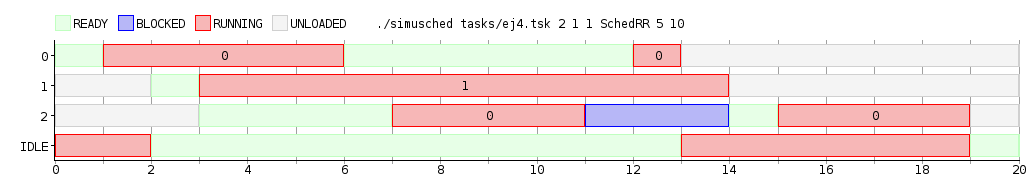
\includegraphics[width=1\columnwidth]{imagenes/ej4.png}
		\caption{\texttt{SchedRR} corriendo 3 tareas con dos núcleos: uno de 5 y
		otro de 10.}
	\end{center}
\end{figure}
